\documentclass[a4paper,12pt]{article}
\usepackage[utf8]{inputenc}
\usepackage[T1]{fontenc}
\usepackage[ngerman]{babel}
\usepackage{geometry}
% Anpassung der Ränder und des Header-Platzes, um fancyhdr-Warnungen zu vermeiden
\geometry{a4paper, left=2.5cm, right=2.5cm, top=3cm, bottom=3cm, headheight=15pt}
\usepackage{fancyhdr}
\usepackage{hyperref}
\usepackage{url}
\usepackage{listings}
\usepackage[dvipsnames]{xcolor}
\usepackage{pdfpages}
\usepackage{graphicx}


\lstset{
   literate={ö}{{\"o}}1
           {ä}{{\"a}}1
           {ü}{{\"u}}1
           {ß}{{\ss}}1
           {é}{{\'e}}1,
   inputencoding=ansinew,
   extendedchars=true,
   basicstyle=\scriptsize\ttfamily,
   numberstyle=\scriptsize,
   breaklines=true,
   tabsize=4,
   numbersep=5pt
}
\lstdefinestyle{textstyle}{
    language={},                 % Verhindert blau markierte Wörter im Text
    basicstyle=\small\sffamily,  % Serifenlose Schrift (Arial-Look)
    breaklines=true,             % Automatischer Zeilenumbruch
    xleftmargin=0pt,             % Absolut keine Einrückung von links
    xrightmargin=0pt,            % Nutzt die volle Breite rechts
    frame=none,                  % Kein Kasten drumherum
    numbers=none,                % Keine Zeilennummern
    keepspaces=true,             % Behält deine Leerzeichen/Formatierung bei
    columns=fullflexible,        % WICHTIG: Erlaubt "normale" Buchstabenabstände
    literate={ä}{{\"a}}1 {ö}{{\"o}}1 {ü}{{\"u}}1 {ß}{{\ss}}1 % Fix für Umlaute
}

\lstdefinestyle{customcpp}{
   language=C++,
   frame=single,
   numbers=left,
   keywordstyle=\color{blue}\bfseries,
   stringstyle=\color{BrickRed}\ttfamily,
   commentstyle=\color{OliveGreen}\ttfamily,
   showspaces=false,
   showstringspaces=false,
   showtabs=false,
   xleftmargin=5px
}

% Setup für Kopf- und Fußzeilen gemäß Vorlage
\pagestyle{fancy}
\fancyhf{} % Löscht Standard-Kopf-/Fußzeilen
\lhead{J. Rieger, L. Kieweg}
\chead{Systemdokumentation}
\rhead{Seite \thepage}
\renewcommand{\headrulewidth}{0.4pt}
\renewcommand{\footrulewidth}{0pt}

\begin{document}

%****************** self defined commands ***************************
%include a .cpp source file
%usage: \cppfile{../path_to_your_file/filename}
\newcommand{\cppfile}[1]{
\begin{itemize}
\item[]\lstinputlisting[label={lst:\detokenize{#1}}, style=customcpp,
    caption=\texttt{\detokenize{#1.cpp}}]{#1.cpp}
\end{itemize}
}

%include a .h source file
%usage: \hfile{../path_to_your_file/filename}
\newcommand{\hfile}[1]{
\begin{itemize}
\item[]\lstinputlisting[label={lst:\detokenize{#1}}, style=customcpp,
    caption=\texttt{\detokenize{#1.h}}
]{#1.h}
\end{itemize}
}

%include a module (.cpp and .h)
%usage: \hfile{../path_to_your_file/filename}
\newcommand{\cppmodul}[1]{
\begin{itemize}
\item[]\lstinputlisting[caption=#1.h,label="lst:#1-header", style=customcpp]{#1.h}
\item[]\lstinputlisting[caption=#1.cpp,label="lst:#1-impl", style=customcpp]{#1.cpp}
\end{itemize}
}

%include a code snippet
%usage: \hfile{../path_to_your_file/filename}{startline}{endline}
\newcommand{\snippet}[3]{
\begin{itemize}
\item[]\lstinputlisting[caption=#1.cpp,label="lst:#1-snip", style=customcpp, firstline=#2,lastline=#3]{#1.cpp}
\end{itemize}
}

%include a test-output file 
%usage: \testoutput{../path_to_your_file/filename}
\newcommand{\testoutput}[1]{
\begin{itemize}
\item[]\lstinputlisting[caption=#1]{#1.txt}
\end{itemize}
}

%include a figure -> ensure that the picture is in the pics directory
%usage: \fig{name_of_picture}{width}{caption text}
%width between 0.0 - 1.0 -> correspond with textwidth
\newcommand{\fig}[3]{
\begin{figure}[H]
\centering
\includegraphics[width=#2\textwidth]{pics/#1.PNG}
\caption{#3}
\label{fig:#1}
\end{figure}
}

\lstset{
   literate={ö}{{\"o}}1
           {ä}{{\"a}}1
           {ü}{{\"u}}1
           {ß}{{\ss}}1
           {é}{{\'e}}1,
   inputencoding=ansinew,
   extendedchars=true,
   basicstyle=\scriptsize\ttfamily,
   numberstyle=\scriptsize,
   breaklines=true,
   tabsize=4,
   numbersep=5pt
}

\lstdefinestyle{customcpp}{
   language=C++,
   frame=single,
   %backgroundcolor=\color{mygray},
   numbers=left,
   keywordstyle=\color{blue}\bfseries,
   stringstyle=\color{BrickRed}\ttfamily,
   commentstyle=\color{OliveGreen}\ttfamily,
   showspaces=false,
   showstringspaces=false,
   showtabs=false,
   xleftmargin=5px
}

% Angabe
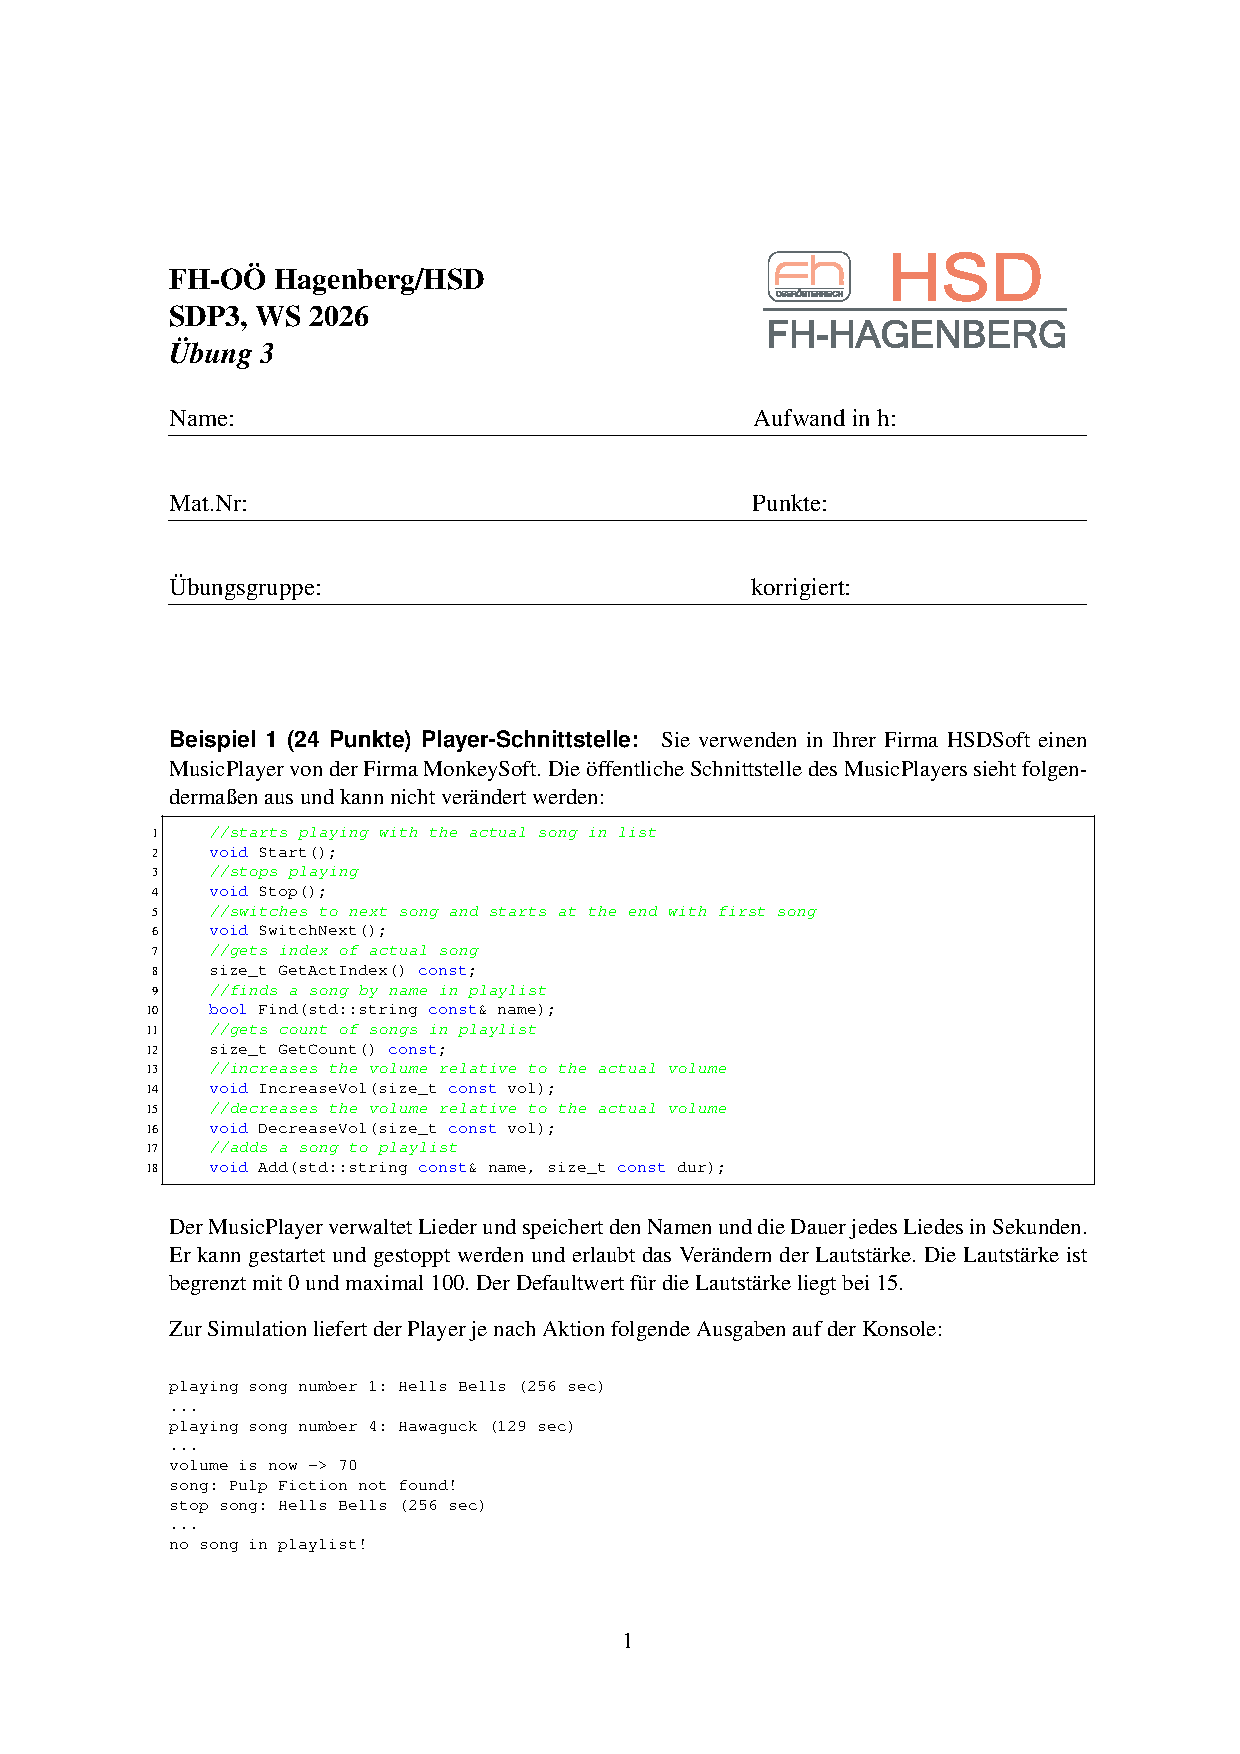
\includepdf[pages=-]{Angabe.pdf}



% -- Titelseite --
\begin{titlepage}
\vspace*{-1cm}
\noindent
HSD\\
OBERÖSTERREICH\\
FH-HAGENBERG

\vspace{4cm}
\begin{center}
{\Huge \textbf{Systemdokumentation}}\\[1cm]
{\Large \textbf{Player-Schnittstelle}}\\[0.5cm]
{\large Version 1.0}\\[2cm]
{\large J. Rieger, L. Kieweg}\\[0.5cm]
{\large Hagenberg, 28. Oktober 2026}
\end{center}

\vspace{3cm}
\noindent
Dieses Dokument zeigt den prinzipiellen Aufbau einer Systemdokumentation für Software-Projekte. Die einzelnen Kapitel sind mit Kommentaren versehen, welche die Struktur und den Inhalt erläutern.
\end{titlepage}

% -- Inhaltsverzeichnis --
\newpage
\tableofcontents
\newpage

% -- Kapitel 1 --
\section{Organisatorisches}
\subsection {Team}
\begin{itemize}
\item Julian Rieger, Matr.-Nr: S2510306023, E-Mail: S2510306023@fhooe.at
\item Leander Kieweg, Matr.-Nr: S2510306014, E-Mail: S2510306014@fhooe.at
\end{itemize}

\subsection{Aufteilung der Verantwortungsbereiche}
\begin{itemize}
\item Julian Rieger
    \begin{itemize}
        \item Implementierung der Klassen: Video, PlayerClient, VideoPlayer, VideoAdapter
        \item Implementierung des Testtreibers
        \item Verfassen der Systemdokumentation
    \end{itemize}
\item Leander Kieweg
    \begin{itemize}
        \item Implementierung der Klassen: Player, MusicAdapter, MusicPlayer, Media, Song
        \item Design des Klassendiagrams
        \item Implementierung des Testtreibers

    \end{itemize}
\end{itemize}

\subsection{Aufwand}
\begin{itemize}
\item Julian Rieger: geschätzt: 7h, tatsächlich 7h
\item Leander Kieweg: geschätzt 7h, tatsächlich 7h
\end{itemize}

\newpage
% -- Kapitel 2 --
\section{Anforderungsdefinition (Systemspezifikation)}
Es wird eine Software zur generischen Bedienung von zwei verschiedenen Schnittstellen, die eines Video Players und die eines Music Players, und stellt eine einzige, für beide verwendbare Schnittstelle, bereit. Die Schnittstelle soll sieben verschiedene Methoden zur Verfügung stellen, die die Geräte steuern können.
\subsection*{Funktionale Anforderungen}
\begin{itemize}
    \item \textbf{Play():} Startet die Wiedergabe des Titels.
    \item \textbf{Stop():} Beendet die Wiedergabe des Titels.
    \item \textbf{Next():} Springt in der Playlist auf den nächsten Titel.
    \item \textbf{Prev():} Springt in der Playlist auf den vorherige Titel.
    \item \textbf{VolInc():} Erhöht die Lautstärke um den Wert 1.
    \item \textbf{VolDec():} Verringert die Lautstärke um den Wert 1.
    \item \textbf{Select(const std::string name):} Wählt einen bestimmten, in der Playlist vorhandenen, Titel aus und startet die Wiedergabe.
\end{itemize}

\subsection*{Fehlerbehandlung}
Fehler bei der Anwendung oder Bedienung des Programms werden abgefangen und es werden Rückmeldungen per std::cerr auf die Konsole ausgegeben und die Funktion wird mit return umgehend wieder verlassen. Zu diese Art von Fehlern zählen jegliche Fehlbedienungen der Schnittstelle. (z.B. Aufruf von Play bei leerer Playlist) Dabei kommt es zu keinen Einschränkungen der darauffolgenden Funktionsaufrufen, sofern ein korrekter Aufruf stattfindet.
\newpage
% -- Kapitel 3 -- 
\section{Systementwurf}
\subsection{Klassendiagramm}

\begin{figure}[htbp]
  \centering
  \makebox[\textwidth][c]{%
    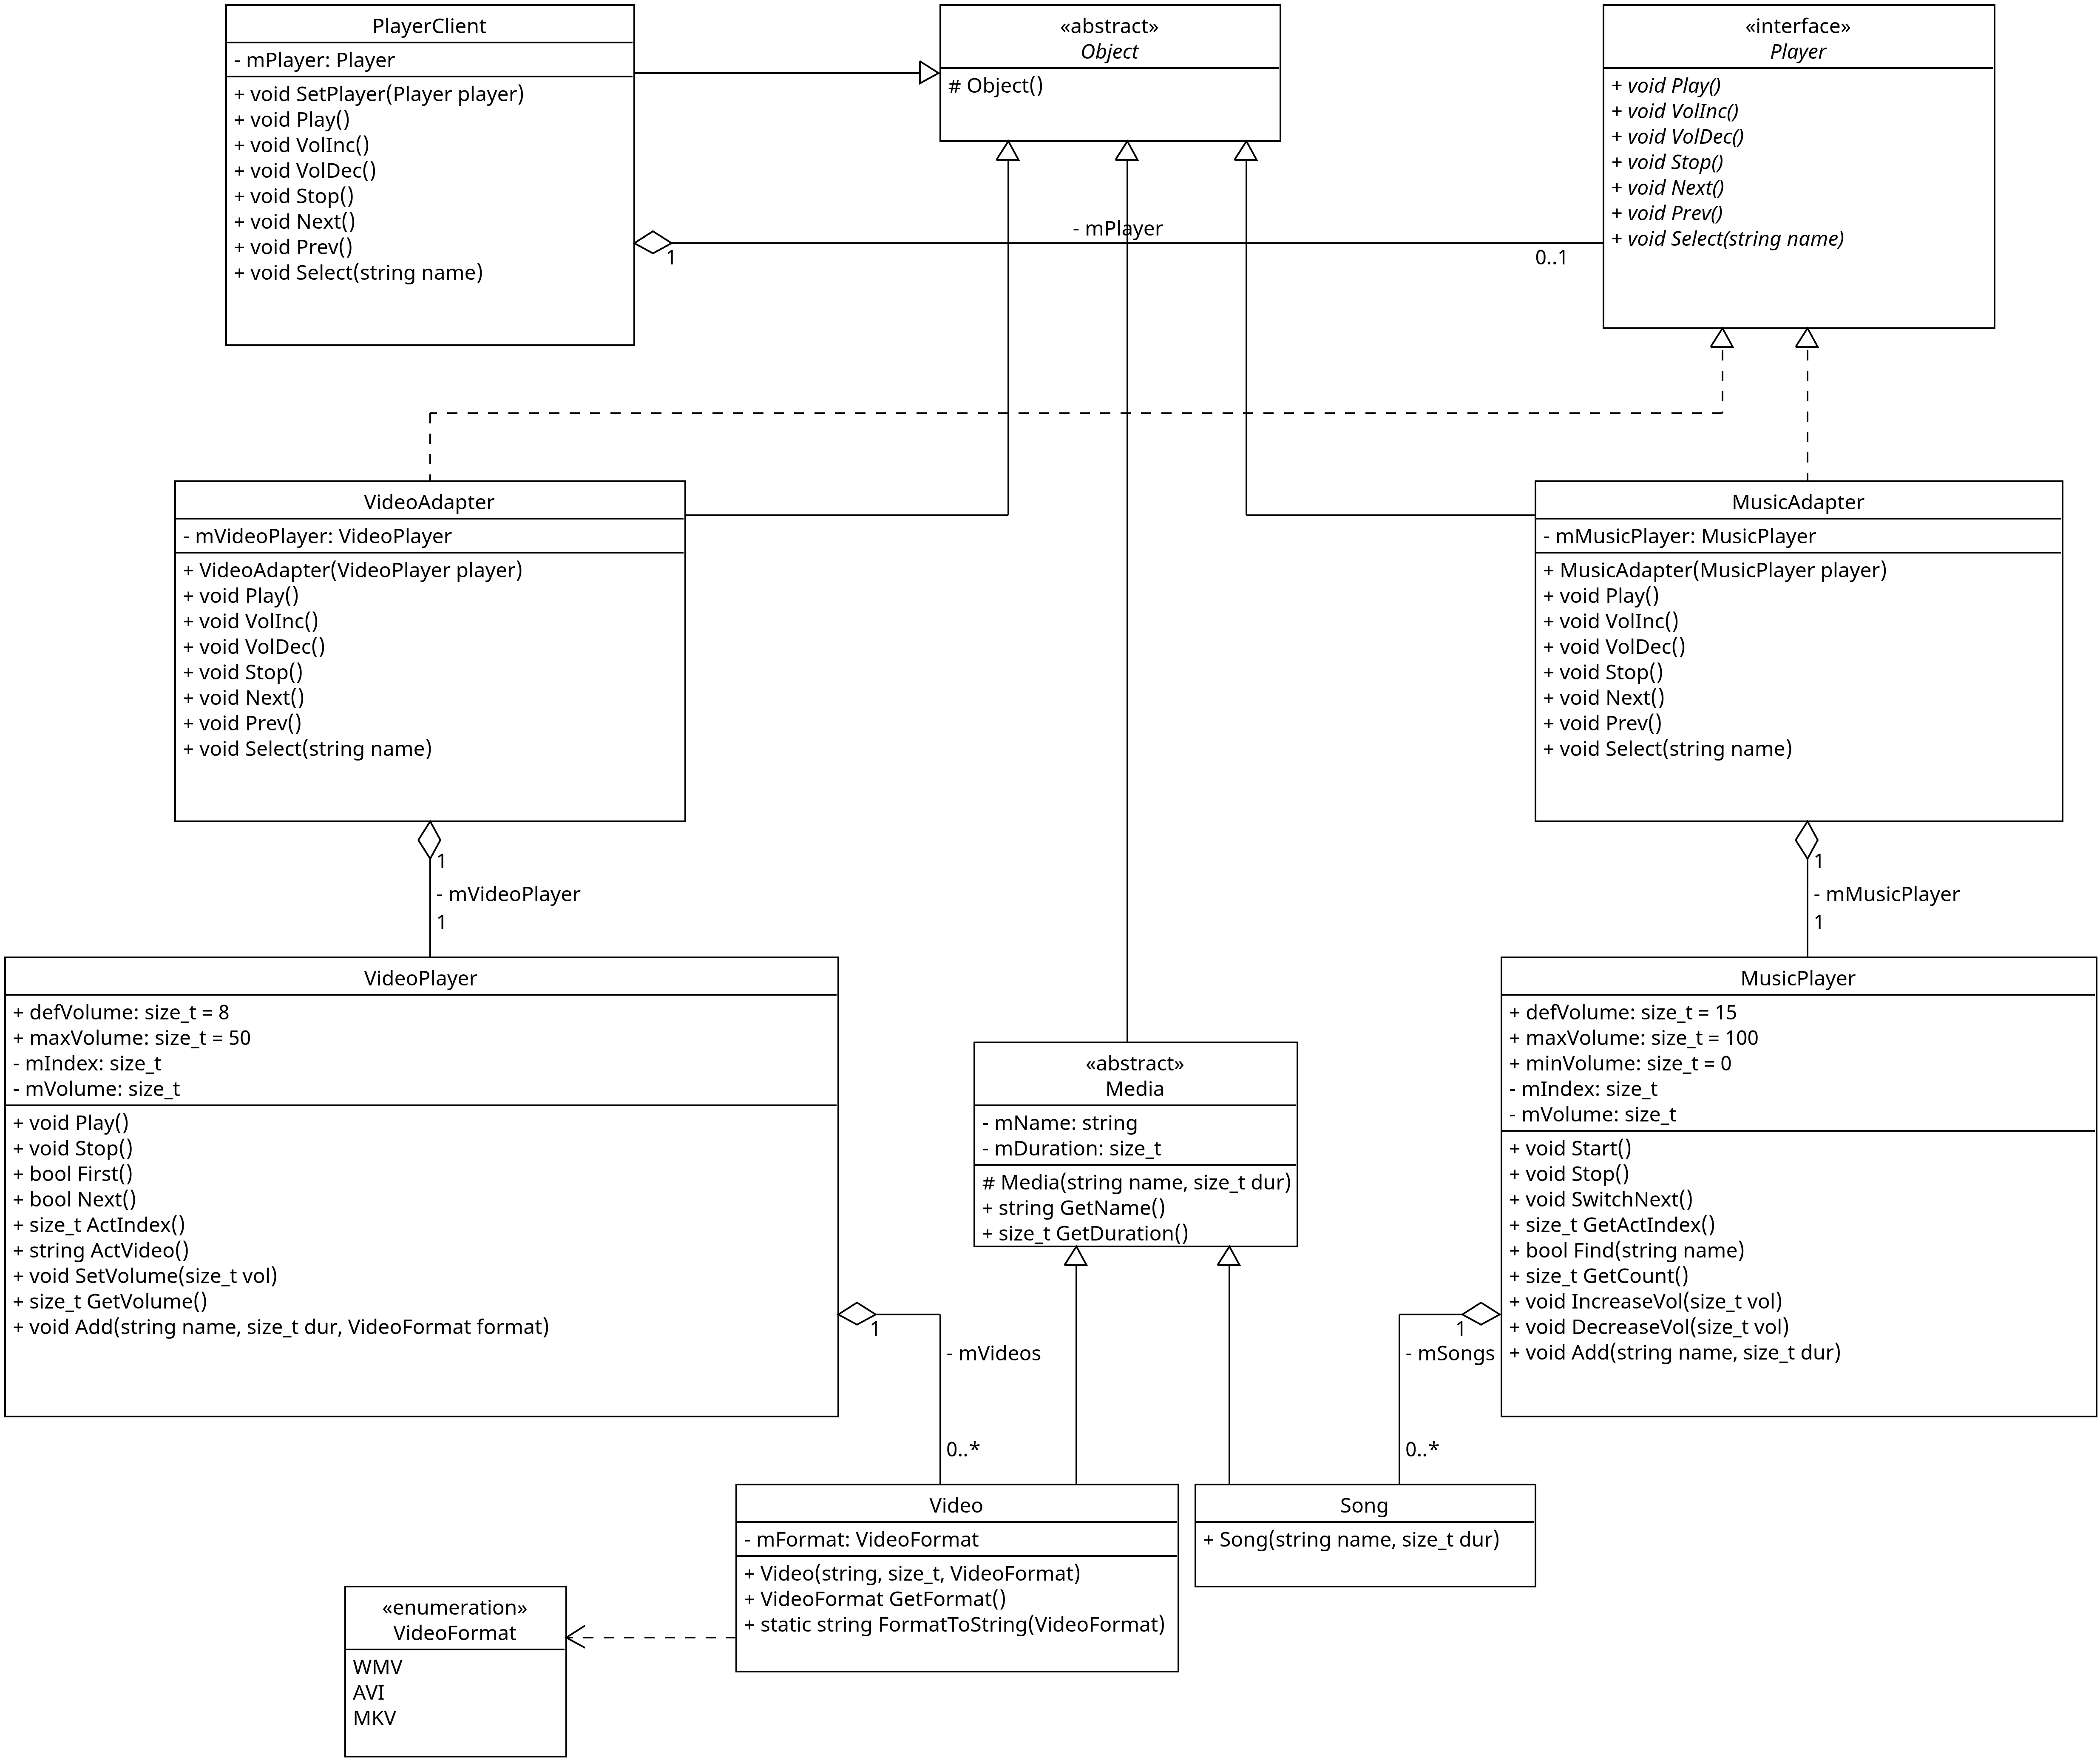
\includegraphics[width=1.0\textwidth]{diagramm.png}% Ohne .png, falls pdflatex genutzt wird
  }%
  \caption{Klassendiagramm Player}
  \label{fig:klassendiagramm}
\end{figure}
Anmerkung: Das Klassendiagram steht für bessere Lesbarkeit ebenfalls im Sysdoku-Ordner zur Verfügung.

\newpage
\subsection{Designentscheidungen}
Für die Konzeption und Implementierung der einheitlichen Player-Schnittstelle wurden gezielt objektorientierte Design-Prinzipien und Entwurfsmuster angewandt, um eine lose Kopplung und hohe Erweiterbarkeit zu garantieren.

\paragraph{Adapter-Pattern}
Da die beiden vorgegebenen Fremdklassen \texttt{VideoPlayer} (von DonkeySoft) und \texttt{MusicPlayer} (von MonkeySoft) unterschiedliche, unveränderliche Schnittstellen besitzen, wurde das \textbf{Adapter-Pattern} eingesetzt. Die Klassen \texttt{VideoAdapter} und \texttt{MusicAdapter} implementieren jeweils das einheitliche \texttt{Player}-Interface und übersetzen die Methodenaufrufe in die jeweilige proprietäre Schnittstelle. Dadurch kann der \texttt{PlayerClient} beide Medientypen über eine gemeinsame, generische Schnittstelle steuern.

\paragraph{Vererbungshierarchie und gemeinsame Basisklassen}
Zur Reduzierung von Code-Duplikaten und für ein sauberes Fundament erben alle zentralen Klassen von einer abstrakten Basisklasse \texttt{Object}. Zudem wurde für die Medienverwaltung die abstrakte Klasse \texttt{Media} eingeführt, von der die Klassen \texttt{Video} und \texttt{Song} abgeleitet sind. Gemeinsame Attribute wie Name und Dauer werden dadurch zentral in \texttt{Media} verwaltet.

\paragraph{Zustandsverwaltung und Kapselung}
Der \texttt{PlayerClient} hält eine optionale Referenz auf ein \texttt{Player}-Interface und delegiert Befehle direkt an diesen. Zur Vermeidung von Nullzeiger-Zugriffen wird im Client stets geprüft, ob ein gültiger Player gesetzt ist. Die spezifischen Restriktionen der Player (unterschiedliche Lautstärkebereiche wie 0--50 beim VideoPlayer bzw. 0--100 beim MusicPlayer) werden innerhalb der jeweiligen Adapter und Player sicher gekapselt und abgefangen.

\paragraph{Fehlerstrategie}
Fehlbedienungen (wie beispielsweise der Versuch, ein Medium bei leerer Playlist abzuspielen) werden kontrolliert abgefangen. Entsprechend den Vorgaben werden aussagekräftige Fehlermeldungen auf der Konsole ausgegeben und die betroffenen Methoden kontrolliert verlassen, ohne das Gesamtsystem zu destabilisieren.

% -- Kapitel 4 --
\section{Komponentenentwurf}
Die HTML-Startdatei befindet sich im Verzeichnis ./../doxy/html/index.html

\newpage
% -- Kapitel 5 --
\section{Testprotokollierung}
\subsection{Ausgabe Konsole Testtreiber}
\begin{lstlisting}[style=textstyle]
--- VideoPlayer ---
volume is now -> 5
Volume verified: 5
Index 0: Video1
playing video number 1: Video1 [duration -> 120 min], WMV-Format
Index 1: Video2
playing video number 2: Video2 [duration -> 90 min], AVI-Format
Index 2: Video3
playing video number 3: Video3 [duration -> 200 min], MKV-Format
stop video: Video3 [duration -> 200 min], MKV-Format
[SUCCESS] VideoPlayer passed

--- MusicPlayer ---
Count verified: 3
volume is now -> 18
volume is now -> 17
playing song number 1: Song1 (180 sec)
Index verified: 1
song: Song9 not found!
stop song: Song3 (150 sec)
[SUCCESS] MusicPlayer passed

--- VideoAdapter via Client ---
playing video number 1: Video1 [duration -> 120 min], WMV-Format
volume is now -> 9
playing video number 2: Video2 [duration -> 90 min], AVI-Format
playing video number 1: Video1 [duration -> 120 min], WMV-Format
playing video number 3: Video3 [duration -> 200 min], MKV-Format
video: NonExisting not found!
stop video: Video3 [duration -> 200 min], MKV-Format
--- MusicAdapter via Client ---
playing song number 1: Song1 (180 sec)
volume is now -> 14
playing song number 2: Song2 (210 sec)
playing song number 1: Song1 (180 sec)
playing song number 2: Song2 (210 sec)
song: NonExisting not found!
stop song: Song2 (210 sec)
[SUCCESS] Adapters passed

--- Edge Cases ---
no video in playlist!
no song in playlist!
[SUCCESS] EdgeCases passed

All tests successfully executed and verified!


\end{lstlisting}

% -- Kapitel 6 --
\newpage
\section{Quellcode}
\hfile{../Object}
\hfile{../Media}
\cppfile{../Media}
\hfile{../Video}
\cppfile{../Video}
\hfile{../Song}
\cppfile{../Song}
\hfile{../VideoPlayer}
\cppfile{../VideoPlayer}
\hfile{../VideoAdapter}
\cppfile{../VideoAdapter}
\hfile{../MusicPlayer}
\cppfile{../MusicPlayer}
\hfile{../MusicAdapter}
\cppfile{../MusicAdapter}
\hfile{../Player}
\hfile{../PlayerClient}
\cppfile{../PlayerClient}
\cppfile{../main}
\end{document}